\documentclass[12pt]{article}
\usepackage{amsmath}
\newcommand{\myvec}[1]{\ensuremath{\begin{pmatrix}#1\end{pmatrix}}}
\newcommand{\mydet}[1]{\ensuremath{\begin{vmatrix}#1\end{vmatrix}}}
\newcommand{\solution}{\noindent \textbf{Solution: }}
\providecommand{\brak}[1]{\ensuremath{\left(#1\right)}}
\providecommand{\norm}[1]{\left\lVert#1\right\rVert}
\let\vec\mathbf
\usepackage{float}
\usepackage{graphicx}

\title{Chapter Name}
\author{Kishan(pusarlakishan@sriprakashschools.com)}

\begin{document}
\maketitle
\section*{10$^{th}$ Maths - Chapter 7}
This is Problem-6.1 from Exercise 7.1
\begin{enumerate}
\item Name the type of quadrilateral formed, if any, by the following points, and give reasons for your answer:  \\ 
(i) (– 1, – 2), (1, 0), (– 1, 2), (– 3,0)\
-2(2)+2(2)\\
-4+4\\
0=0\\

so, it is a parallelogram\\

if $\brak{\vec{A}-\vec{C}}^{\top}\brak{\vec{B}-\vec{D}}=0$ then it is a rhombus\\
$\myvec{0&0}{\myvec{4\\0}}$\\
0(4)-0(0)\\
0-0\\
0 = 0\\

so, it is a rhombus\\

if $\brak{\vec{A}-\vec{D}}^{\top}\brak{\vec{A}-\vec{B}}=0$ then it is a square\\
$\myvec{2&2}^{\top}{\myvec{-2\\2}}$\\
2(-2)+2(2)\\
-4+4\\
0= 0\\

so, it is a square\\

if $\brak{\vec{A}-\vec{B}}^{\top}\brak{\vec{B}-\vec{C}}=0$ then it is a rectangle\\
$\myvec{-2&2}^{\top}{\myvec{2\\-2}}$\\
-2(2)+2(-2)\\
-4+4\\
0=0\\

so, it is a rectangle\\ 
It is a square because every square is rectangle,rhombus and parallelogram
\end{enumerate}
\begin{figure}[H]
			\centering
			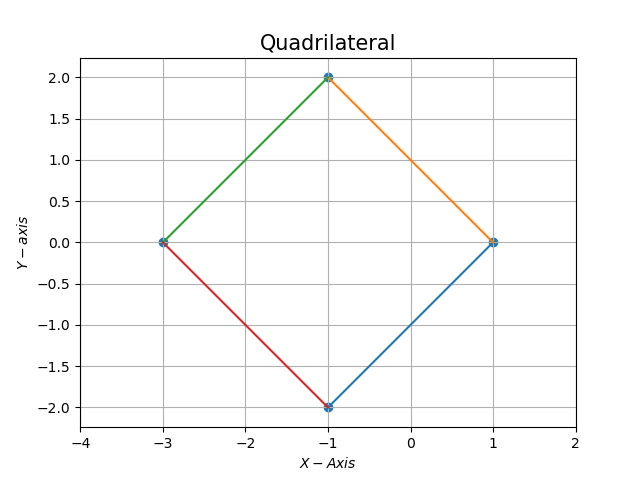
\includegraphics[width=\columnwidth]{figs/Figure_1.png}
			\caption{Quadrilateral ABCD}
			\label{fig:16}
		\end{figure}
\end{document}
